\documentclass[12pt, a4paper, twoside]{article}

%% Preamble
\usepackage[spanish,es-tabla]{babel}
\usepackage{umatfgspanish}
\usepackage{blindtext}
\usepackage{biblatex}
\usepackage{comment}
\usepackage{float}
\usepackage{subfig}
\usepackage{multirow}
\usepackage{longtable}
\usepackage{minted}
\usepackage{tabularx}
\usepackage{listings}
\usepackage{xcolor} % to access the named colour LightGray



\usepackage{pgfplots}
 
\pgfplotsset{compat = newest}



\definecolor{LightGray}{gray}{0.98}



\addbibresource{bibliography.bib}

\graphicspath{{images/}{../images/}}

\usepackage{subfiles} % Best loaded last in the preamble

\begin{document}

%% Cover
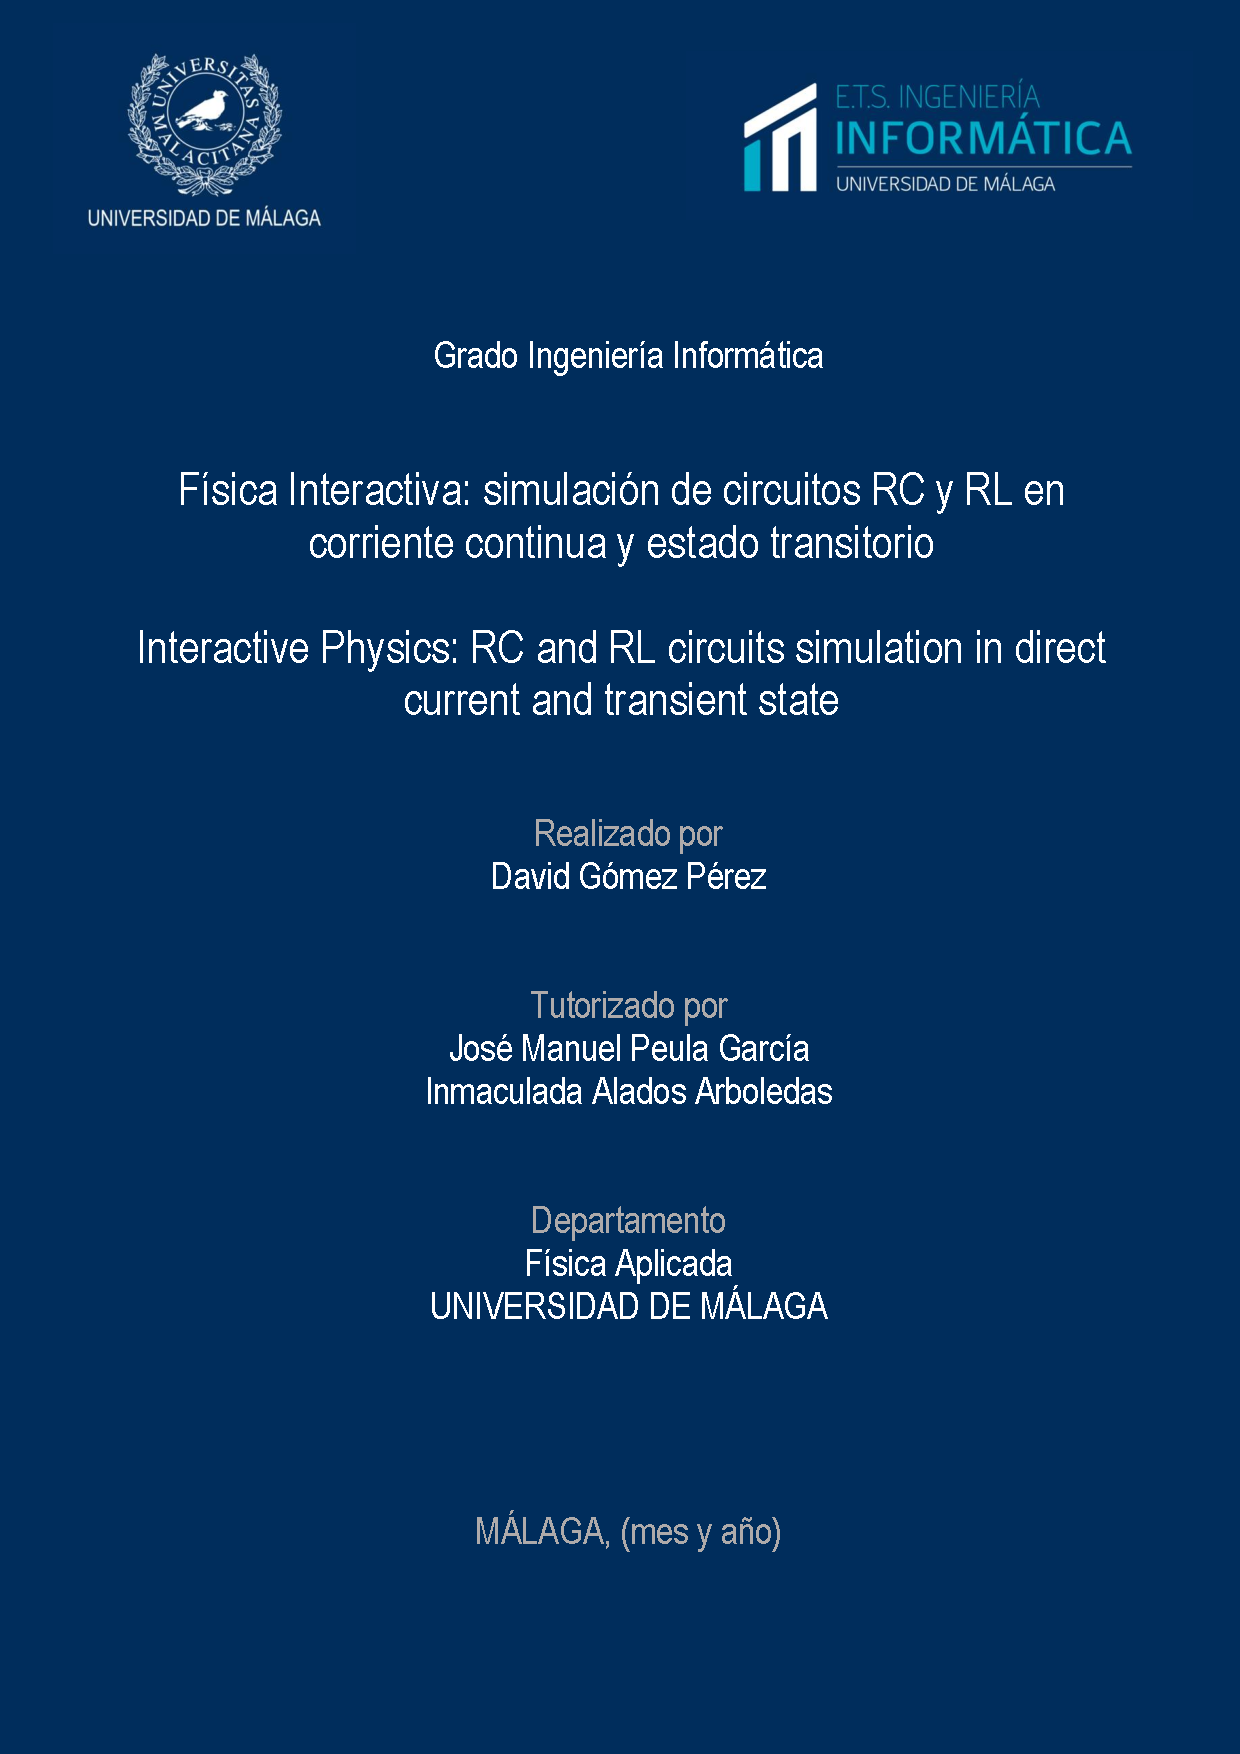
\includepdf[noautoscale=true, width=\paperwidth]{cover.pdf}

%% Title
\clearpage
\setcounter{page}{1}


\includepdf[noautoscale=true, width=\paperwidth]{title.pdf}

\newpage

%% Abstract
\subfile{sections/abstract}

\newpage

\subfile{sections/resumen}

\tableofcontents

%% Sections
\section{Introducción}
\subfile{sections/introduccion}

\section{Circuitos RC y RL}
\subfile{sections/circuitosRCyRL}

\section{Estudio de las tecnologías}
\subfile{sections/tecnologias}

\section{Implementación y pruebas}
\subfile{sections/implementacion}

\section{Conclusions and Futures Lines of Research}
\subfile{sections/conclusion}

\section{Conclusiones y Líneas Futuras}
\subfile{sections/conclusiones}


%% Bibliography
\printbibliography

\newpage

%% Apendices
\begin{umaappendices}
  \section{Manual de instalación y de usuario}
  \subfile{sections/manual_instalacion}
\end{umaappendices}


\begin{umaappendices}
  \section{Requisitos y casos de uso}
  \subfile{sections/requisitos_casos_uso}
\end{umaappendices}


\begin{umaappendices}
  \section{Modelado de los circuitos RC y RL}
  \subfile{sections/resumen_ecuaciones}
\end{umaappendices}

\begin{umaappendices}
  \section{Resolución matemática del circuito RC}
  \subfile{sections/resolucionEcuaciones}
\end{umaappendices}

\begin{umaappendices}
  \section{Resolución matemática del circuito RL}
  \subfile{sections/resolucionEcuaciones2}
\end{umaappendices}



%% Back Cover

\includepdf[noautoscale=true, width=\paperwidth]{backcover.pdf}
\end{document}
